% !TEX root = ../../../main.tex
% 来源：高中物理甲种本·第一册（力学）
% 章节：机械能 / 动能
% 原始文件：7.tex，行 261-272
% 类型：tikz
% ---
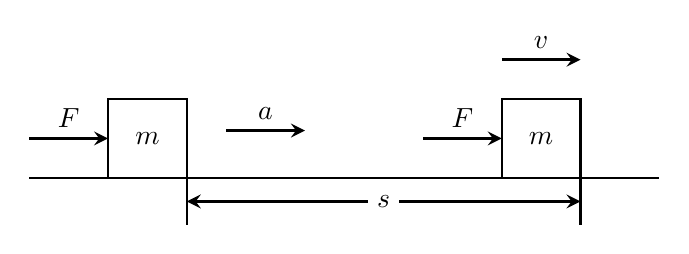
\begin{tikzpicture}[>=stealth, thick]
\draw (0,0)--(8,0);
\draw (1,0) rectangle (2,1);  \draw (6,0) rectangle (7,1);
\node at (1.5,.5){$m$}; \node at (6.5,.5){$m$};
\draw[->, very thick](0,.5)--node [above]{$F$}(1,.5);  \draw[->, very thick](5,.5)--node [above]{$F$}(6,.5);
\draw[->, very thick](2.5,.6)--node [above]{$a$}(3.5,.6);
\draw[->, very thick](6,1.5)--node [above]{$v$}(7,1.5);
\draw (2,0)--(2,-.6);
\draw (7,0)--(7,-.6);
\draw[<->, very thick](2,-.3)--node [fill=white]{$s$}(7,-.3);

\end{tikzpicture}
